% Recommended PET Configuration: Comparison with Gregor's Implementation
% Editable source for the deck. Build: pdflatex -interaction=nonstopmode <this file>
% Every number carries a source; the claim-to-evidence index is
% ../CLAIM_EVIDENCE_INDEX-20260918.md and the full inventory is
% ../CONFIGURATION_COMPARISON-20260918.md.
\documentclass[aspectratio=169,10pt]{beamer}
\usetheme{default}
\usecolortheme{seahorse}
\setbeamertemplate{navigation symbols}{}
\setbeamertemplate{footline}[frame number]
\setbeamerfont{frametitle}{size=\large}
\setbeamercolor{frametitle}{fg=black}
\usepackage[T1]{fontenc}
\usepackage[utf8]{inputenc}
\usepackage{booktabs}
\usepackage{array}
\usepackage{xcolor}
\usepackage{graphicx}
\definecolor{ours}{HTML}{1F4E79}
\definecolor{theirs}{HTML}{A6611A}
\definecolor{warn}{HTML}{8B0000}
\newcommand{\ours}[1]{\textcolor{ours}{#1}}
\newcommand{\theirs}[1]{\textcolor{theirs}{#1}}
\newcommand{\warn}[1]{\textcolor{warn}{#1}}
\newcommand{\src}[1]{{\scriptsize\color{gray}\texttt{#1}}}
\newcolumntype{R}[1]{>{\raggedright\arraybackslash}p{#1}}
\setlength{\tabcolsep}{4pt}
\renewcommand{\arraystretch}{1.12}

\title{Recommended PET Configuration}
\subtitle{Comparison with Gregor's Implementation}
\author{Publication Agent B (PET)}
\date{18 September 2026}

\begin{document}

% ---------------------------------------------------------------- 1
\begin{frame}
  \titlepage
  \begin{center}
    \small
    \warn{PET is diagnostic method development, not a publication product.}\\
    \small Nothing here is a publication adoption, an uncertainty, or a Gate-6 action.
  \end{center}
\end{frame}

% ---------------------------------------------------------------- 2
\begin{frame}{Executive recommendation}
  \textbf{Keep our estimator's structure. Borrow five things from Gregor. Test two of
  them before anything else.}
  \vspace{0.6em}

  \begin{columns}[T]
    \begin{column}{0.49\textwidth}
      \ours{\textbf{Keep} (evidence supports, or load-bearing for OmniFold)}
      \begin{itemize}\small
        \item muon as a distinguished FiLM event input
        \item frozen MC normalization; periodic azimuth
        \item family pooling as the practical default
        \item energy-ranked retention
        \item KNN locality in detector coordinates
        \item the whole OmniFold construction
      \end{itemize}
    \end{column}
    \begin{column}{0.49\textwidth}
      \theirs{\textbf{Borrow} (candidates --- none deployed)}
      \begin{itemize}\small
        \item \textbf{per-family log energy sums}, computed over the whole event
        \item \textbf{aggregate overflow}, energy-weighted merge
        \item richer per-token features + type embedding
        \item warmup + cosine decay, gradient clipping
        \item one capacity step
      \end{itemize}
    \end{column}
  \end{columns}
  \vspace{0.5em}
  \hrule
  \vspace{0.4em}
  {\small
  \textbf{Do first, zero new compute:} measure whether typed objects cover the
  cluster energy. That one number gates the three largest borrowings.\\
  \textbf{Do not borrow:} muon-as-token; zero-fill for absent fields; embedding index
  0 shared with padding; input LayerNorm; raw $\phi$; concatenation-order truncation;
  weight decay.}
\end{frame}

% ---------------------------------------------------------------- 3
\begin{frame}{What is pinned, and what ``ours'' means}
  \begin{center}\footnotesize
  \begin{tabular}{@{}R{0.20\textwidth}R{0.40\textwidth}R{0.34\textwidth}@{}}
    \toprule
    \textbf{label} & \textbf{what it is} & \textbf{pin} \\
    \midrule
    \ours{ours, production} &
      \texttt{pet-fullevent-fps-v1}: the estimator the driver stamps &
      \texttt{44142e8c} (branch \texttt{pet-direct-token-comparison}) \\
    \ours{ours, experimental} &
      four-arm representation study: typed descriptors, routing, aggregate overflow.
      \warn{No arm is in the production path.} &
      \texttt{44142e8c}, \texttt{direct\_token\_comparison/} \\
    \ours{ours, proposed} &
      what this deck recommends changing &
      \warn{nothing is built} \\
    \theirs{Gregor's} &
      \texttt{gregorkrz/minerva-ml} &
      \texttt{fc9a099d}, 2026-07-20, clean tree \\
    \bottomrule
  \end{tabular}
  \end{center}
  \vspace{0.5em}
  \begin{itemize}\small
    \item \warn{\texttt{fc9a099} is the repo as cloned, not a paper commit.} No release
      tags; the repo has evolved past arXiv:2604.12364. The paper commit must come
      from Gregor.
    \item Everything attributed to him is the \textbf{default} unless marked optional.
      Verified at \texttt{fc9a099}: \texttt{use\_pid} on, \texttt{use\_cond} on,
      \texttt{include-E-sum} on, \texttt{max\_particles} 33,
      \warn{\texttt{use-max-blobs-and-prongs} \emph{off}} --- so his overflow
      aggregation is optional and not the default.
    \item \textbf{He is not doing unfolding.} Supervised regression/classification, MC
      only, no data leg, no per-event weights. Several rows below have no counterpart,
      and that is a difference in problem, not in quality.
  \end{itemize}
\end{frame}

% ---------------------------------------------------------------- 4
\begin{frame}{The actual baseline: our production estimator}
  \begin{columns}[T]
    \begin{column}{0.52\textwidth}
      {\small\textbf{Data path}}
      \begin{itemize}\footnotesize
        \item cloud $=$ \textbf{raw non-muon calorimeter clusters}
          $(E,\mathrm{pos},z,\mathrm{view},t)$, 5 columns
        \item muon \textbf{removed from the cloud}; carried as a 13-feature event block,
          FiLM conditioning
        \item cap: stable energy sort, \textbf{top 12}, zero-pad ---
          applied \warn{at dump time}, so changing it needs a re-dump
        \item overflow \textbf{discarded with no trace}: no count, no summed energy, no flag
        \item fixed physical divisors; event features z-normalized with \emph{frozen}
          reco-MC \texttt{pass\_reco} statistics
        \item azimuth as $(\cos\phi,\sin\phi)$ everywhere
      \end{itemize}
    \end{column}
    \begin{column}{0.46\textwidth}
      {\small\textbf{Model and training}}
      \begin{itemize}\footnotesize
        \item PET: encoder $\to$ \textbf{KNN local aggregation} ($K=3$ over
          $(\mathrm{pos},z)$) $\to$ 2 blocks, 2 heads, width 32, LayerScale $\to$
          class token + FiLM head
        \item \textbf{47{,}041 trainable parameters}; 93{,}954 per OmniFold iteration
        \item weighted BCE; Adam $10^{-4}$ annealed to $10^{-5}$, realized LR
          \emph{asserted} at runtime; batch 512; niter 3, epochs 8; 2\,M subsample
        \item MultiFold; push weight $w=\exp(\mathrm{logit})$ in logit space
        \item background: negweight-refined, fail-closed
        \item seed 42 frozen --- this is what makes $C_{\rm stat}$ statistical
      \end{itemize}
    \end{column}
  \end{columns}
  \vspace{0.3em}
  \src{train\_fullevent\_nominal.py:403-407, 47-71; fullevent\_fps\_dataloader.py;
       dump\_pointcloud\_inputs.py:90-112; omnifold\_nn/omnifold/\{net,omnifold\}.py;
       receipts/model-capacity.json}
\end{frame}

% ---------------------------------------------------------------- 5
\begin{frame}{Gregor's implementation}
  \begin{columns}[T]
    \begin{column}{0.52\textwidth}
      {\small\textbf{Data path}}
      \begin{itemize}\footnotesize
        \item cloud $=$ \textbf{reconstructed objects}: muon, $\le 2$ photons, blobs,
          prongs --- 10 columns each
        \item $\eta$, $\phi$, $\log p_T$, $\log E$, \textbf{PID code} (8-class learned
          embedding), $dE/dx$, $x,y,z,t$ (all $/10^4$)
        \item muon is \textbf{a token like any other} (PID 0)
        \item caps in series: 150 at preprocessing (energy-sorted \emph{only} if
          exceeded), then \warn{first 33 rows at batch time, no re-sort}
        \item absent fields \warn{zero-filled, no validity mask}
        \item 16 global features: recoil calorimetry, passive material, Michel, $\gamma\gamma$
          mass, prong count, \textbf{6 per-PID log energy sums}
      \end{itemize}
    \end{column}
    \begin{column}{0.46\textwidth}
      {\small\textbf{Model and training}}
      \begin{itemize}\footnotesize
        \item \texttt{PointGlobalMixedViT}: mixed encoder $\to$ \textbf{Fourier
          positional MLP over $(\eta,\phi)$} $\to$ 4 pre-norm blocks, 8 heads,
          $d_{\rm model}=128$ $\to$ CLS fused with EVT token
        \item \textbf{890{,}130 parameters --- $18.9\times$ ours}
        \item Huber on $\log 1p$; \textbf{AdamW}, wd 0.01, \textbf{1000-step warmup then
          cosine}, \textbf{grad clip 1.0}; batch 2048; 100k--500k steps
        \item optional: OmniLearned PET2, HyperScale, BERT, pretrained init
        \item \warn{pretrained checkpoints are unreachable} --- HyperScale repo 404,
          NERSC URLs time out (audit \texttt{B\_provenance})
      \end{itemize}
    \end{column}
  \end{columns}
  \vspace{0.3em}
  \src{vit.py:226-373; train.py:465-756, 2328-2358; preprocessing.py:257-583;
       jobs/submit\_train\_jobs.py:150-151; gregor-audit/jobs/A\_dataset.out.md}
\end{frame}

% ---------------------------------------------------------------- 6
\begin{frame}{Comparison I --- representation}
  \begin{center}\scriptsize
  \begin{tabular}{@{}R{0.135\textwidth}R{0.215\textwidth}R{0.215\textwidth}R{0.175\textwidth}R{0.175\textwidth}@{}}
    \toprule
    & \ours{\textbf{ours}} & \theirs{\textbf{Gregor's}} & \textbf{consequence} &
      \textbf{recommendation} \\
    \midrule
    objects &
      raw non-muon calorimeter clusters; muon distinguished &
      reconstructed objects; muon is a token &
      mean 74.6/102.6 clusters vs 14.0/15.6 objects: $5.3\times$/$6.6\times$ fewer tokens &
      \theirs{borrow} the vocabulary; \ours{keep} the distinguished muon \\
    token features &
      5 cols, no type code; mask $=(E{=}0)$ &
      10 cols incl.\ direction, $dE/dx$, time, PID embedding &
      more physics per object; but zero-fill hides absence, and padding shares PID
      index 0 with muon (masked, so latent) &
      \theirs{borrow} features + embedding; \warn{reserve index 0 for padding} \\
    transforms &
      physical divisors; frozen MC z-norm; $(\cos\phi,\sin\phi)$ &
      logs $+/10^4$; LayerNorm inside encoder; \warn{raw $\phi$} &
      raw $\phi$ is discontinuous at the wrap --- we fixed this ourselves in July &
      \ours{keep} ours; recommend the $\phi$ fix to him \\
    event globals &
      13, all muon/vertex &
      16, recoil calorimetry + \textbf{6 per-PID energy sums} &
      his sums are a fixed-width channel that survives a cap --- but he computes them
      \emph{after} truncation &
      \theirs{borrow} the sums, computed \emph{before} any cap \\
    caps and overflow &
      top 12 by energy, rest discarded silently &
      150 then first 33 unsorted; aggregate token \emph{optional, off} &
      our cap binds $64\%$/$84\%$ vs his $9$--$17\%$/$11$--$27\%$; his ordering is worse &
      \theirs{borrow} aggregation; \ours{keep} energy ranking \\
    \bottomrule
  \end{tabular}
  \end{center}
\end{frame}

% ---------------------------------------------------------------- 7
\begin{frame}{Comparison II --- model, training, integration}
  \begin{center}\scriptsize\renewcommand{\arraystretch}{1.0}
  \begin{tabular}{@{}R{0.135\textwidth}R{0.215\textwidth}R{0.215\textwidth}R{0.175\textwidth}R{0.175\textwidth}@{}}
    \toprule
    & \ours{\textbf{ours}} & \theirs{\textbf{Gregor's}} & \textbf{consequence} &
      \textbf{recommendation} \\
    \midrule
    routing &
      one family, so no question in production; pooled vs individual measured
      experimentally &
      individual, unconditionally &
      no accuracy difference detected; individual costs $1.24\times$ at the operating
      point, $1.88\times$ in the tail &
      \ours{keep} pooling as a practical default \\
    architecture &
      2 blocks, 2 heads, width 32, KNN in $(\mathrm{pos},z)$; \textbf{47k params} &
      4 blocks, 8 heads, width 128, Fourier PE in $(\eta,\phi)$; \textbf{890k params} &
      $18.9\times$ gap; ours is retrained $\sim$130 times per campaign, his once &
      \ours{keep} architecture; treat capacity as \textbf{open} \\
    init &
      random, seed 42 frozen (this makes $C_{\rm stat}$ statistical) &
      random; optional pretrained OmniLearned &
      \warn{checkpoints unreachable}: 404 and timeouts &
      \ours{keep}; ask Gregor for the weights and hashes \\
    training &
      Adam $10^{-4}\!\to\!10^{-5}$ step anneal; no wd, no clip &
      AdamW, wd 0.01, warmup + cosine, clip 1.0 &
      his schedule is better conditioned and free; \warn{wd biases a likelihood-ratio
      classifier} ($w=e^{\rm logit}$) &
      \theirs{borrow} warmup/cosine/clip; \warn{not} weight decay \\
    OmniFold &
      full MultiFold, logit-space ratio, negweight background, fail-closed data
      path; closures PASS &
      \warn{no counterpart} --- MC only, no weights, no flags &
      his \emph{dataset} cannot be an OmniFold input; his \emph{vocabulary} can &
      \ours{keep} ours in full \\
    \bottomrule
  \end{tabular}
  \end{center}
  \vspace{0.1em}
  {\scriptsize \warn{Before any numeric comparison with his results:} his $E_{\rm avail}$
  uses full charged-pion energy $+$ $K^{\pm}$ against our pion-KE definition ---
  an offset of order 140\,MeV per $\pi^{\pm}$.}
\end{frame}

% ---------------------------------------------------------------- 8
\begin{frame}{The measured problem: our cap binds, and it binds hard}
  \begin{center}
    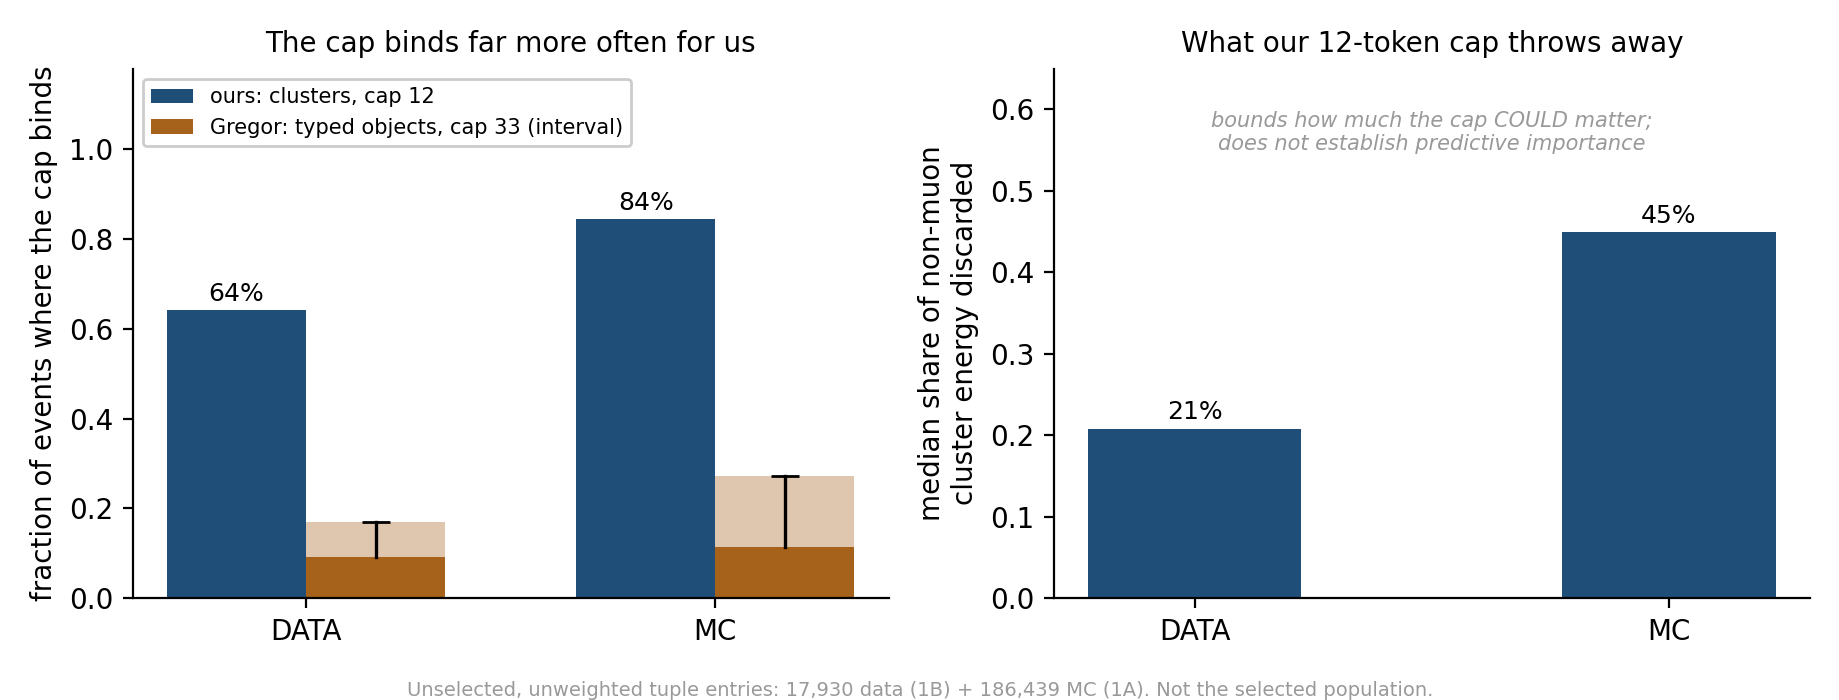
\includegraphics[width=0.88\textwidth]{figures/fig-cap.png}
  \end{center}
  \vspace{-0.6em}
  {\scriptsize
  Same two tuple files, both vocabularies. Our 12-token cluster cap binds in
  \textbf{64.1\,\% (data) / 84.4\,\% (MC)} of events and discards a median
  \textbf{20.8\,\% / 44.9\,\%} of non-muon cluster energy. A 33-token typed-object cap
  binds in \textbf{9.2--16.9\,\% / 11.4--27.2\,\%} --- an interval, because the receipt
  holds marginal, not joint, family multiplicities.
  \\[0.2em]
  \warn{Three things this does not show.} It does not show the discarded clusters carry
  predictive information. It does not predict a closure improvement --- \textbf{no
  closure measurement of aggregation exists}. And these are \textbf{unselected,
  unweighted} tuple entries, so they do not determine selected-population behaviour.}
  \\[0.2em]
  \src{receipts/typed-object-budget.json; source-multiplicity.json (job 58470099)}
\end{frame}

% ---------------------------------------------------------------- 9
\begin{frame}{Measured accuracy and stability: routing is inconclusive}
  \begin{columns}[T]
    \begin{column}{0.52\textwidth}
      {\footnotesize Eight paired seeds, four-object synthetic fixture, information
      content / model size / budget / init / seeds held identical between arms.}
      \begin{center}\footnotesize
      \begin{tabular}{@{}lr@{}}
        \toprule
        paired improvement, individual over pooled & \\
        \midrule
        median & $+9.7\,\%$ \\
        mean & $+0.8\,\%$ \\
        seed-to-seed sd & $25.8$ points \\
        95\,\% interval on the mean & $[-20.7,\,+22.4]\,\%$ \\
        paired $p$ & $0.50$ \\
        favourable seeds & 6 of 8 \\
        \bottomrule
      \end{tabular}
      \end{center}
      {\footnotesize Frozen decision: \textbf{\texttt{NO\_PASS}}, 142 of 146 checks
      holding. Two failures \emph{were} the inconclusive result; separately
      \texttt{shuffle-71} missed two projection checks marginally (0.0119 vs 0.01;
      absolute errors well inside 0.05).}
    \end{column}
    \begin{column}{0.46\textwidth}
      {\footnotesize\textbf{What each number measures} ---}
      \begin{itemize}\footnotesize
        \item the interval is on the \textbf{mean paired injected-improvement percentage
          across training seeds on a synthetic fixture}. Not on production closure, not
          on real data.
        \item $p=0.50$ is a paired test \textbf{across training seeds}. It measures
          seed scatter. \warn{Test-sample uncertainty was not separately estimated.}
        \item 25.8 points is a \textbf{planning assumption} carried from a different
          fixture, two arms and a different denominator --- \warn{not measured power for
          the endpoint now specified.}
      \end{itemize}
      {\footnotesize\warn{And: in the fixture every generic slot is noise while in
      production the cluster cloud carries most of the information. Neither direction
      nor magnitude of a synthetic effect transfers automatically.}}
    \end{column}
  \end{columns}
\end{frame}

% ---------------------------------------------------------------- 10
\begin{frame}{Measured cost: what each change actually buys and spends}
  \begin{center}
    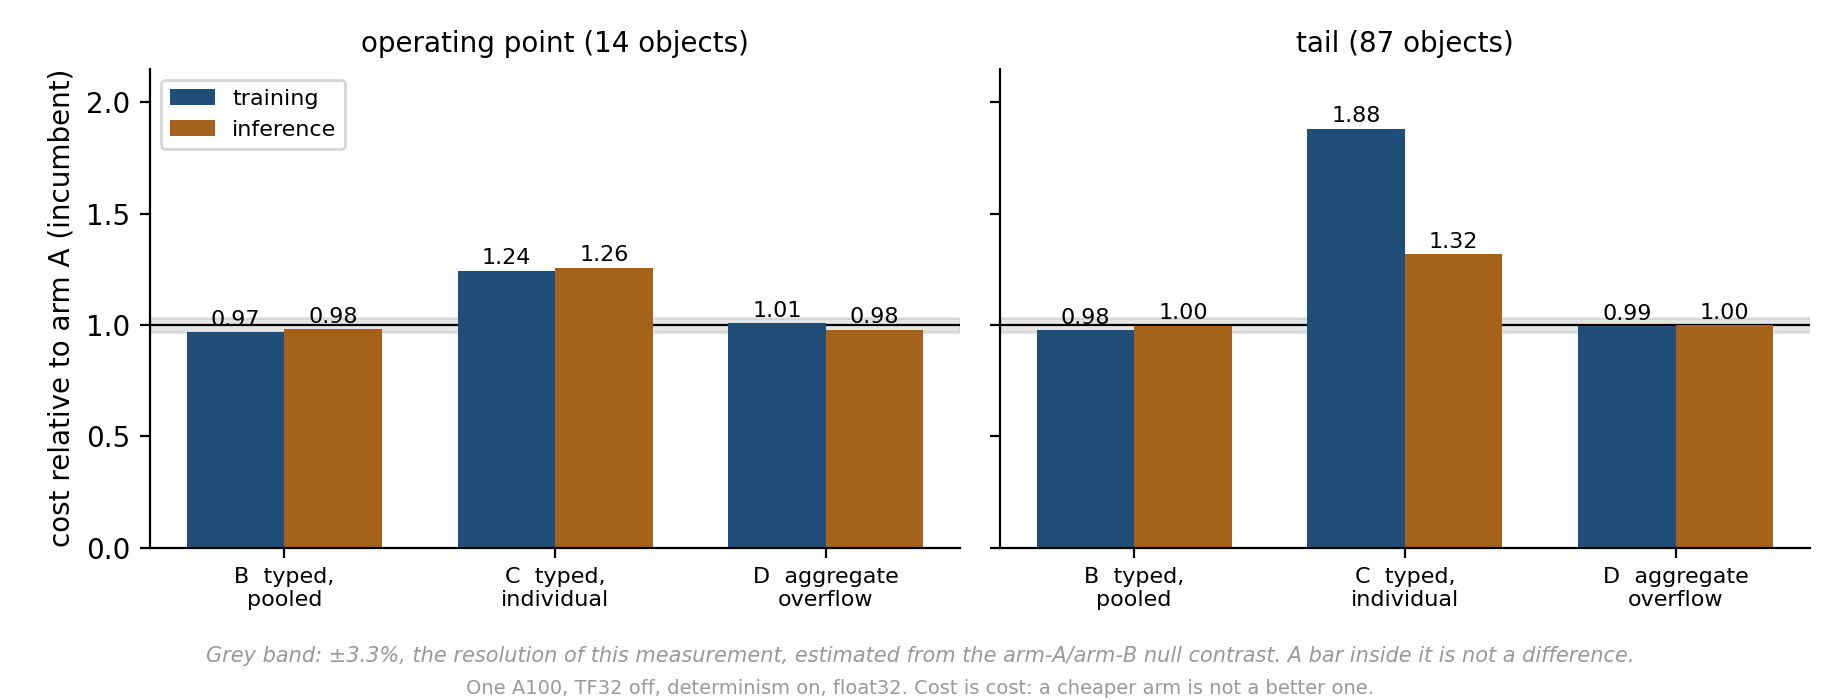
\includegraphics[width=0.84\textwidth]{figures/fig-cost.png}
  \end{center}
  \vspace{-0.7em}
  {\scriptsize
  \textbf{Aggregate overflow is \emph{not} free --- it is indistinguishable from parity
  at this measurement's resolution.} Arm B is computationally identical to arm A in the
  pooled configuration and still reads $0.97\times$, so the floor is about
  $\pm3.3\,\%$. The non-compute cost is real: a dump regeneration, a schema field, a
  re-validation, and a new estimator fingerprint.
  \\[0.2em]
  \textbf{Individual routing is outside that band and grows with multiplicity}
  ($1.24\times \to 1.88\times$ training). Pooling is nearly flat. Our campaign
  multiplier is $\sim$130 trains, so per-train cost is multiplied, not absorbed.}
  \\[0.2em]
  \src{cost-half.json (one A100, TF32 off, determinism on, float32); inference-benchmark.json}
\end{frame}

% ---------------------------------------------------------------- 11
\begin{frame}{Retained, borrowed, deferred}
  \begin{center}\scriptsize
  \begin{tabular}{@{}R{0.30\textwidth}R{0.20\textwidth}R{0.20\textwidth}R{0.24\textwidth}@{}}
    \toprule
    \textbf{borrow (candidate)} & \textbf{why} & \textbf{measured cost} &
      \textbf{prerequisite} \\
    \midrule
    per-family log energy sums, over the \emph{whole} event &
      cap-proof fixed-width channel &
      $\approx$ 0 &
      fingerprint change; rank alongside \texttt{eavail}/\texttt{q3} \\
    aggregate overflow, energy-weighted merge &
      addresses a measured 21--45\,\% energy loss in most events &
      parity to $\pm3.3\,\%$ &
      dump regeneration; \warn{no closure evidence yet} \\
    richer per-token features + type embedding, index 0 reserved &
      more physics per token, fewer tokens &
      unmeasured &
      \warn{typed-object energy coverage} \\
    warmup + cosine, gradient clipping &
      better-conditioned schedule &
      $\approx$ 0 &
      Gate-4 fingerprint; closure re-run \\
    one capacity step &
      $18.9\times$ gap is a live hypothesis &
      multiplies through the UQ campaign &
      price against the campaign, not one train \\
    \bottomrule
  \end{tabular}
  \end{center}
  \vspace{0.4em}
  {\footnotesize
  \textbf{Deferred, deliberately:} individual-object routing --- unresolved on accuracy
  and measurably more expensive. \textbf{Decided without new work:} normalization,
  pretraining availability, OmniFold integration, numerical behaviour.
  \\[0.2em]
  \textbf{Back to Gregor:} encode $\phi$ periodically; reserve embedding index 0 for
  padding; map raw prong PID 9 (it currently raises); compute the per-PID energy sums
  before truncation.}
\end{frame}

% ---------------------------------------------------------------- 12
\begin{frame}{Limitations --- what these numbers do not say}
  \begin{enumerate}\small
    \item \warn{``Negligible measured overhead'' is not ``free''.} Aggregate overflow is
      inside the $\pm3.3\,\%$ resolution of the cost measurement, and it carries a
      dump regeneration, a schema change, a re-validation and a new fingerprint.
    \item \warn{Discarded energy does not establish closure improvement.} 21--45\,\%
      bounds how much the cap \emph{could} matter. No closure measurement of aggregation
      exists on either side.
    \item \warn{Validation is incomplete: 10 of 13 widths released.} Three widths failed
      the finite-difference check V5 and were not released. Diagnosis: the
      \emph{criterion} was wrong, not the gradient --- error falls as $h^2$
      ($1.8\!\times\!10^{-2}$ at the frozen $h{=}10^{-2}$, $3.1\!\times\!10^{-4}$ at
      $10^{-3}$) then rises, the signature of truncation giving way to cancellation.
      \textbf{The criterion was not relaxed after the failures.}
    \item \warn{Unselected source measurements do not determine selected behaviour.}
      Two files, unweighted, no production selection, no POT weighting.
    \item \warn{Every statistical quantity is labelled by what it measures} --- seed
      scatter, not test-sample uncertainty; a synthetic fixture, not production; a
      planning assumption, not measured power.
    \item \warn{The pin is the repo, not the paper.} \texttt{fc9a099} may not be what
      produced arXiv:2604.12364.
  \end{enumerate}
\end{frame}

% ---------------------------------------------------------------- 13
\begin{frame}{The next decision}
  \textbf{One question, no compute, gates the three largest borrowings:}
  \begin{center}\small
    Do blobs $+$ prongs $+$ photons cover the non-muon cluster energy on our tuples?
  \end{center}
  {\footnotesize A counts-and-energies read of branches the A1 authorization already
  covers; order one CPU core-hour. If coverage is poor, the typed vocabulary is dead and
  the list collapses to aggregate overflow alone.}
  \vspace{0.6em}
  \hrule
  \vspace{0.5em}
  {\small\textbf{Then one bounded proposal, not five experiments.} Aggregation, energy
  sums, routing and capacity \emph{interact}: energy sums partly substitute for
  aggregation; routing matters more when more objects survive the cap; and a
  47k-parameter model may have no room for a richer representation, which would make
  every single-factor test read ``no effect'' for the wrong reason. The right instrument
  is a \textbf{matched complete-configuration comparison} --- production against one
  assembled candidate on the same endpoint and seeds --- with single-factor arms added
  only where it shows an effect.}
  \vspace{0.5em}
  \hrule
  \vspace{0.5em}
  {\small\textbf{Already authorized and currently blocked.} The variance pilot
  ($\le$30 GPU-h) would measure whether any of this is resolvable inside the 130
  authorized. Its precondition is complete validation, which is unmet. \textbf{One
  decision unblocks it:} amend the frozen V5 criterion to a per-coordinate step rule.
  That is Joseph's call, and I did not make it.}
  \vspace{0.4em}

  {\footnotesize Campaign spend to date: \textbf{16.0 of 290 GPU device-hours}, 2.0 CPU
  core-hours.}
\end{frame}

% ================================================================ appendix
\appendix

\begin{frame}{Appendix A --- claim-to-evidence index}
  \begin{center}\scriptsize
  \begin{tabular}{@{}R{0.40\textwidth}R{0.55\textwidth}@{}}
    \toprule
    \textbf{claim} & \textbf{evidence} \\
    \midrule
    cap binds 64.1\,\% / 84.4\,\%; median 20.8\,\% / 44.9\,\% energy discarded &
      \texttt{direct\_token\_comparison/local\_validation/20260918-source/\allowbreak source-multiplicity.json}
      (job 58470099; 17{,}930 data + 186{,}439 MC entries) \\
    typed cap binds 9.2--16.9\,\% / 11.4--27.2\,\%; $5.3\times$/$6.6\times$ fewer tokens &
      \texttt{receipts/typed-object-budget.json} (derived; 8 tests) \\
    47{,}041 vs 890{,}130 parameters &
      \texttt{receipts/model-capacity.json} (both models instantiated) \\
    routing: median $+9.7\,\%$, $[-20.7,+22.4]\,\%$, $p=0.50$, \texttt{NO\_PASS} 142/146 &
      \texttt{local\_validation/20260917-matrix/matrix-summary.json} \\
    inference $1.283\times$, all 5 checks pass, CV $\le$ 2\,\% &
      \texttt{local\_validation/20260917-inference/inference-benchmark.json} \\
    GPU cost by arm; A/D parity; $\pm3.3\,\%$ floor &
      \texttt{local\_validation/20260918-a3-cost/cost-half.json} \\
    10 of 13 widths released, no hard stop &
      \texttt{local\_validation/20260918-tailval/validation-final.json};
      criteria sha256 \texttt{abccd88b\ldots} \\
    Gregor token format, PID scheme, caps, globals &
      \texttt{gregor-audit/jobs/A\_dataset.out.md} (line-cited to \texttt{fc9a099}) \\
    checkpoints unreachable; OmniLearned MIT; dataset CC-BY-4.0 &
      \texttt{gregor-audit/jobs/B\_provenance.out.md} \\
    our production configuration &
      \texttt{FULL\_EVENT\_FEATURE\_CONTRACT.md};
      \texttt{train\_fullevent\_\allowbreak nominal.py:47-71, 403-407} \\
    \bottomrule
  \end{tabular}
  \end{center}
  {\scriptsize Full index: \texttt{../CLAIM\_EVIDENCE\_INDEX-20260918.md}. Full
  inventory: \texttt{../CONFIGURATION\_COMPARISON-20260918.md}.}
\end{frame}

\begin{frame}[t]{Appendix B --- the V5 diagnosis, in full}
  \vspace{0.4em}
  {\footnotesize Three widths --- $(0,64,2)$ and $(2,160,12)$ for the individual arm,
  $(2,12,4)$ for both --- failed the finite-difference check, and only that check. My
  first hypothesis (a small denominator) was \textbf{wrong}: the failing coordinates
  have $|\nabla| \approx 0.0215$. Sweeping the step at the worst coordinate:}
  \vspace{-0.2em}
  \begin{center}\footnotesize
  \begin{tabular}{@{}rrr@{}}
    \toprule
    $h$ & numeric derivative & relative error \\
    \midrule
    $3\times10^{-2}$ & $-0.01787$ & $1.69\times10^{-1}$ \\
    $1\times10^{-2}$ \emph{(frozen)} & $-0.02111$ & $1.84\times10^{-2}$ \\
    $3\times10^{-3}$ & $-0.02147$ & $1.67\times10^{-3}$ \\
    $1\times10^{-3}$ & $-0.021497$ & $\mathbf{3.14\times10^{-4}}$ \\
    $3\times10^{-4}$ & $-0.021531$ & $1.30\times10^{-3}$ \\
    \bottomrule
  \end{tabular}
  \end{center}
  \vspace{-0.3em}
  {\footnotesize Error falls as $h^2$ and then rises: truncation giving way to cancellation.
  The analytic gradient is correct; the frozen \emph{global} step was too large at those
  coordinates, and the optimal step is per-coordinate. The plateau check nearly caught
  it (16.8\,\% spread against a 20\,\% tolerance).
  \\[0.4em]
  \textbf{I did not relax the criterion.} Releasing those widths requires an amended
  step rule. Until then the execution path is validated for 10 of 13 widths, which is
  \warn{incomplete}, and the variance pilot's precondition is unmet.}
\end{frame}

\begin{frame}{Appendix C --- what the campaign cost, and what it did not authorize}
  \begin{center}\small
  \begin{tabular}{@{}lrl@{}}
    \toprule
    item & GPU device-hours & source \\
    \midrule
    representation matrix (24 paired jobs) & 13.27 &
      \texttt{matrix-summary.json} \\
    A3 geometry probe + width gate (5 subs) & 0.43 &
      \texttt{GO\_NO\_GO-20260918.md} \S7 \\
    tail validation (4 of 4 submissions) & 0.77 of 1.5 authorized &
      \texttt{validation-final.json} \\
    inference benchmark + matrix closeout & \emph{not itemized here} & --- \\
    A1 source characterization & (CPU: 2.0 core-h) & \texttt{source-multiplicity.json} \\
    \midrule
    \textbf{campaign total} & \textbf{16.0 of 290} &
      \texttt{RECOMMENDATION-20260918.md} \\
    \bottomrule
  \end{tabular}
  \end{center}
  \vspace{0.3em}
  {\footnotesize \warn{The first three rows are itemized from their own receipts; the
  total is carried from the campaign recommendation. They do not sum, because the
  inference benchmark (including one 35-minute timeout that measured nothing) and the
  matrix closeout are inside the total but are not separately itemized in any receipt I
  can cite. Stated as a gap rather than closed by arithmetic.}
  \\[0.5em]
  \textbf{Not launched:} the variance pilot ($\le$30 GPU-h, precondition unmet) and
  Stage 2 ($\le$130 GPU-h, downstream of the pilot).
  \\[0.3em]
  \textbf{Not authorized by anything in this deck:} publication adoption, any covariance
  or systematic, a central-value change, a Gate-6 action, or the construction of
  $C_{\rm ML}$. Typed objects and aggregate overflow remain \emph{prospective}
  representation improvements, exactly as the analysis note already says.
  \\[0.3em]
  \textbf{Not done:} nothing in this deck has been sent to anyone.}
\end{frame}

\end{document}
